\setcounter{page}{2}

\textbf{В данной работе будет выполнен 6 вариант.}

\captionsetup{singlelinecheck = false, justification=raggedright}
\begin{lstlisting}[label=code, caption=Код host\_main.cpp]
#include <iostream>
#include <stdio.h>
#include <stdexcept>
#include <iomanip>
#ifdef _WINDOWS
#include <io.h>
#else
#include <unistd.h>
#endif


#include "experimental/xrt_device.h"
#include "experimental/xrt_kernel.h"
#include "experimental/xrt_bo.h"
#include "experimental/xrt_ini.h"

#include "gpc_defs.h"
#include "leonhardx64_xrt.h"
#include "gpc_handlers.h"

#define BURST 128

union uint64 {
	uint64_t 	u64;
	uint32_t 	u32[2];
	uint16_t 	u16[4];   
	uint8_t 	u8[8];   
};

typedef struct adr{  
	uint8_t 	u8[4];   
} adr_t;

uint64_t rand64() {
	uint64 tmp;
	tmp.u32[0] =  rand();
	tmp.u32[1] =  rand();
	return tmp.u64;
}

static void usage()
{
	std::cout << "usage: <xclbin> <sw_kernel>\n\n";
}

int main(int argc, char** argv)
{
	
	
	uint16_t val;
	uint64 valad;
	printf("imput addt:\n");
	scanf("%d.%d.%d.%d", &(valad.u16[0]), &(valad.u16[1]), &(valad.u16[2]), &(valad.u16[3]));
	val = (valad.u16[2] - 32) * 256 + valad.u16[3];
	
	uint16_t n;
	printf("input number:\n");
	scanf("%d", &n);
	
	
	__foreach_core(group, core) {
		lnh_inst.gpc[group][core]->mq_send(val);
		lnh_inst.gpc[group][core]->mq_send(n);
	}
	
	printf("out\n");
	// __foreach_core(group, core) {
		// 	lnh_inst.gpc[group][core]->buf_read(count[group][core]*2*sizeof(uint64),(char*)gpc2host_buffer[group][core]);
		// }
	
	// __foreach_core(group, core) {
		// 	lnh_inst.gpc[group][core]->buf_read_join();
		// }

	// uint64 val;
	// printf("input addr:\n");
	// scanf("%d %d %d %d", &(val.u16[0]), &(val.u16[1]), &(val.u16[2]), &(val.u16[3]));
	uint16_t vaaa;
	__foreach_core(group, core) {
		vaaa = lnh_inst.gpc[group][core]->mq_receive();
		printf("sch 1: %d\n", vaaa);
		vaaa = lnh_inst.gpc[group][core]->mq_receive();
		printf("sch 2: %d\n", vaaa);
		vaaa = lnh_inst.gpc[group][core]->mq_receive();
		printf("sch 3: %d\n", vaaa);
		vaaa = lnh_inst.gpc[group][core]->mq_receive();
		printf("sch 4: %d\n", vaaa);
	}
	
	
	__foreach_core(group, core) {
		free(host2gpc_buffer[group][core]);
		//free(gpc2host_buffer[group][core]);
	}
	
	
	return 0;
}

\end{lstlisting}

\newpage
\begin{lstlisting}[label=code, caption=Код sw\_kernel\_main.cpp]
/*
* gpc_test.c
*
* sw_kernel library
*
*  Created on: April 23, 2021
*      Author: A.Popov
*/ 

#include <stdlib.h>
#include <unistd.h>
#include "lnh64.h"
#include "gpc_io_swk.h"
#include "gpc_handlers.h"

#define SW_KERNEL_VERSION 26
#define DEFINE_LNH_DRIVER
#define DEFINE_MQ_R2L
#define DEFINE_MQ_L2R
#define __fast_recall__

#define TEST_STRUCTURE 1

extern lnh lnh_core;
extern global_memory_io gmio;
volatile unsigned int event_source;


// union uint64 {
	//     uint64_t 	u64;
	//     uint32_t 	u32[2];
	//     uint16_t 	u16[4];   
	//     uint8_t 	u8[8];   
	// };


int main(void) {
	/////////////////////////////////////////////////////////
	//                  Main Event Loop
	/////////////////////////////////////////////////////////
	//Leonhard driver structure should be initialised
	lnh_init();
	//Initialise host2gpc and gpc2host queues
	gmio_init(lnh_core.partition.data_partition);
	for (;;) {
		//Wait for event
		while (!gpc_start());
		//Enable RW operations
		set_gpc_state(BUSY);
		//Wait for event
		event_source = gpc_config();
		switch(event_source) {
			/////////////////////////////////////////////
			//  Measure GPN operation frequency
			/////////////////////////////////////////////
			case __event__(insert_burst) : insert_burst(); break;
			case __event__(search_burst) : search_burst(); break;
		}
		//Disable RW operations
		set_gpc_state(IDLE);
		while (gpc_start());
		
	}
}


void insert_burst() {
	
	lnh_del_str_sync(TEST_STRUCTURE);
	unsigned int count = mq_receive();
	unsigned int size_in_bytes = count*(sizeof(uint16_t));
	uint16_t *buffer = (uint16_t*)malloc(size_in_bytes);
	buf_read(size_in_bytes, (char*)buffer);
	for (int i=0; i<count; i++) {
		lnh_ins_sync(TEST_STRUCTURE, buffer[i], 0);
	}
	lnh_sync();
	free(buffer);
}


void search_burst() {
	
	lnh_sync(); 
	unsigned int count = lnh_get_num(TEST_STRUCTURE);
	uint16_t ip = mq_receive();
	uint8_t n = mq_receive();
	//mq_send(ip);
	uint64 val;
	
	if (lnh_search(TEST_STRUCTURE,ip)) {
		val.u64 = lnh_core.result.value;
		val.u16[n]++;
		lnh_ins_async(TEST_STRUCTURE,ip,val.u64);
	} else {
		val.u64 = 0ull;
		val.u16[n]++;
		lnh_ins_async(TEST_STRUCTURE,ip,val.u64);
	}
	mq_send(val.u16[0]);
	mq_send(val.u16[1]);
	mq_send(val.u16[2]);
	mq_send(val.u16[3]);
}

\end{lstlisting}

Изображение работы программы:

\begin{figure}[h!]
	\begin{center}
		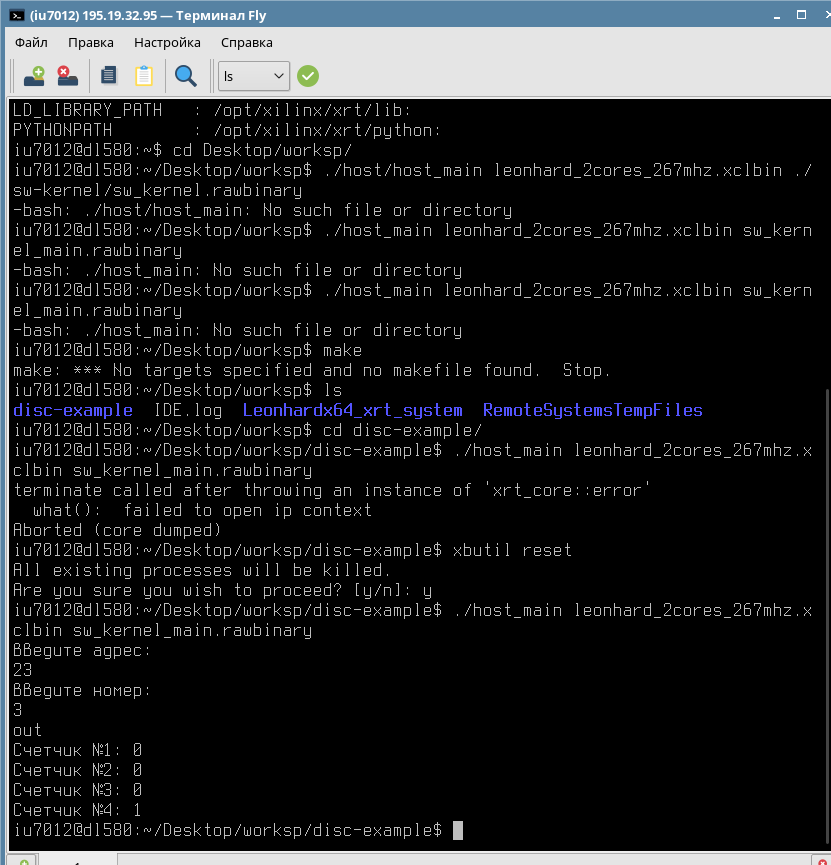
\includegraphics[scale=0.6]{assets/pract1.png}
	\end{center}
\end{figure}